\subsection{Giới thiệu}
Bộ dữ liệu NSL-KDD \cite{nslkdd}, được đề xuất để giải quyết một số vấn đề cố hữu của tập dữ liệu KDD CUP'99.
\par
KDD CUP’99 là bộ dữ liệu được sử dụng rộng rãi nhất để phát hiện bất thường trong máy học.
Nhưng Tavallaee và cộng sự đã tiến hành một phân tích thống kê về tập dữ liệu này và tìm thấy hai vấn đề quan trọng ảnh hưởng rất lớn đến hiệu năng của các hệ thống được đánh giá và kết quả đánh giá rất kém về các phương pháp phát hiện bất thường.
Để giải quyết những vấn đề này, họ đề xuất một bộ dữ liệu mới, NSL-KDD, bao gồm các bản ghi đã chọn của bộ dữ liệu KDD hoàn chỉnh.
\newline
\par
Sau đây là những ưu điểm của NSL-KDD so với bộ dữ liệu KDD gốc:
\par
\begin{itemize}
	\item Đầu tiên, nó không bao gồm các bản ghi dự phòng trong huấn luyện, vì vậy các bộ phân loại sẽ không bị thiên vị đối với các bản ghi thường xuyên hơn.
	\item Thứ hai, số lượng các bản ghi được chọn từ mỗi nhóm mức độ khó tỷ lệ nghịch với tỷ lệ phần trăm của các bản ghi trong bộ dữ liệu KDD gốc.
	      Kết quả là, tỷ lệ phân loại của các phương pháp học máy riêng biệt khác nhau ở phạm vi rộng hơn, làm cho nó nhiều hiệu quả hơn để có một đánh giá chính xác về các kỹ thuật học tập khác nhau.
	\item Thứ ba, số lượng hồ sơ trong tập huấn và kiểm tra là hợp lý, điều này làm cho nó hợp lý để chạy thử nghiệm trên bộ hoàn chỉnh mà không cần phải chọn ngẫu nhiên một phần nhỏ. Do đó, kết quả đánh giá của các công trình nghiên cứu khác nhau sẽ nhất quán và có thể so sánh được.
\end{itemize}
\subsection{Đặc tính}
\begin{figure}[!htbp]
	\centering
	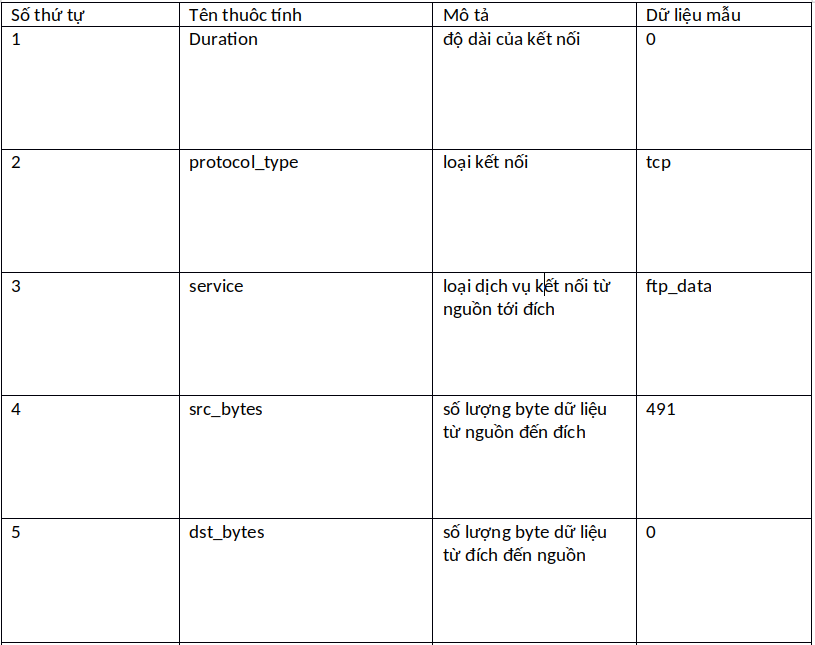
\includegraphics[scale=0.5]{table1}
	\label{fig:x cubed graph}
\end{figure}
\FloatBarrier
\begin{figure}[!htbp]
	\centering
	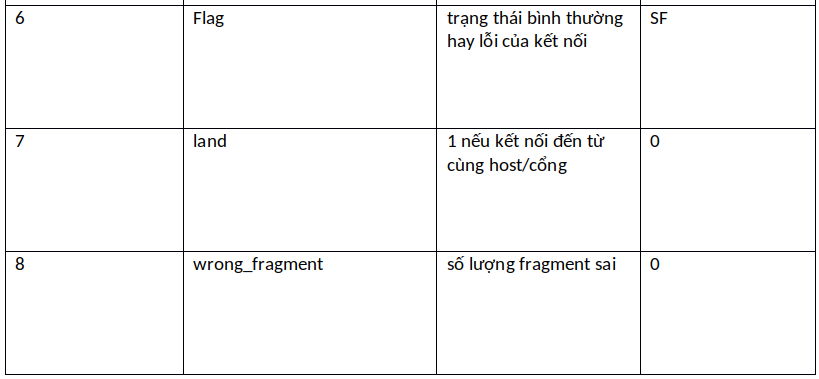
\includegraphics[scale=0.5]{table2}
	\label{fig:x cubed graph}
\end{figure}
\FloatBarrier
\begin{figure}[!htbp]
	\centering
	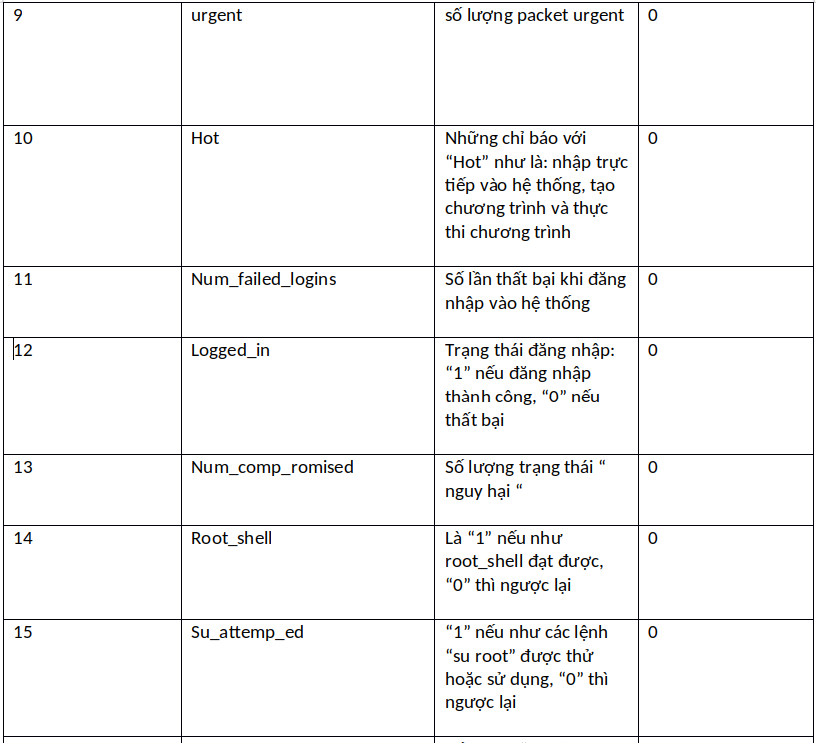
\includegraphics[scale=0.5]{table3}
	\label{fig:x cubed graph}
\end{figure}
\FloatBarrier
\begin{figure}[!htbp]
	\centering
	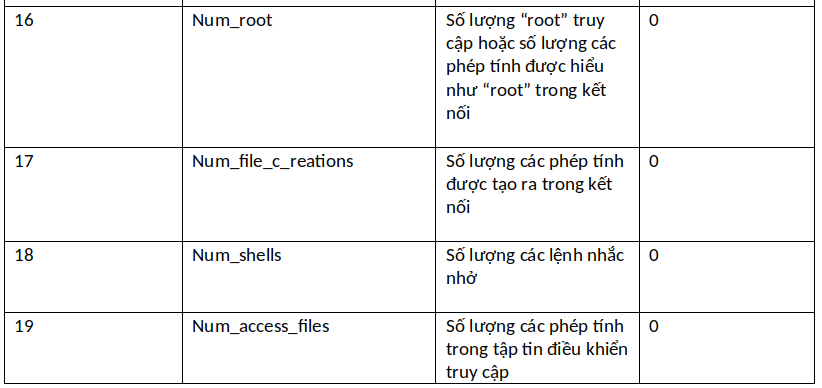
\includegraphics[scale=0.5]{table4}
	\label{fig:x cubed graph}
\end{figure}
\FloatBarrier
\begin{figure}[!htbp]
	\centering
	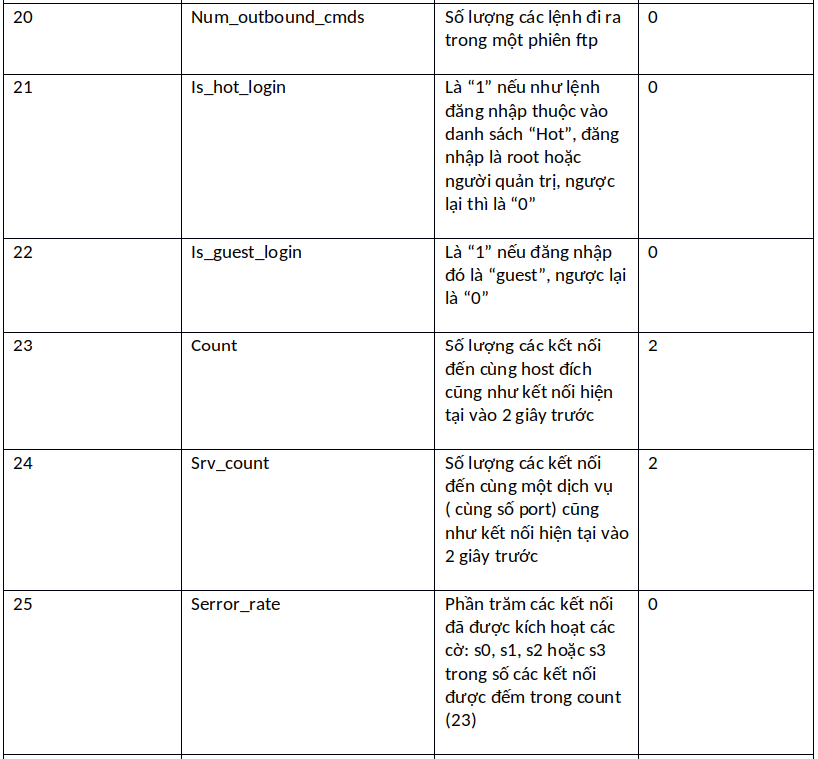
\includegraphics[scale=0.5]{table5}
	\label{fig:x cubed graph}
\end{figure}
\FloatBarrier
\begin{figure}[!htbp]
	\centering
	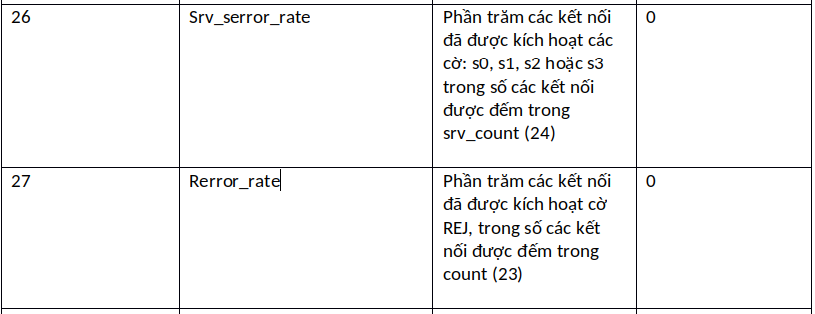
\includegraphics[scale=0.5]{table6}
	\label{fig:x cubed graph}
\end{figure}
\FloatBarrier
\begin{figure}[!htbp]
	\centering
	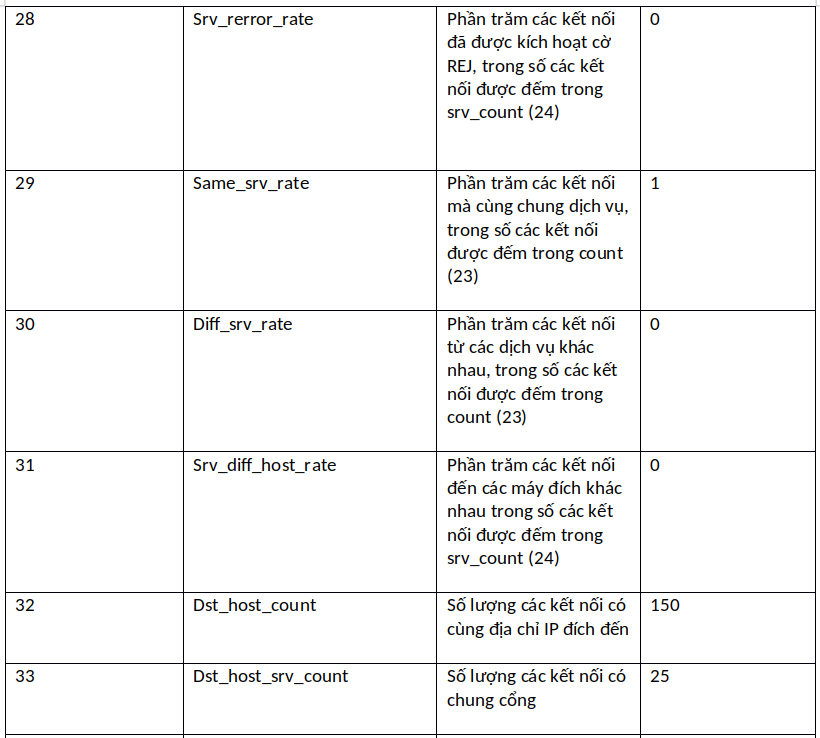
\includegraphics[scale=0.5]{table7}
	\label{fig:x cubed graph}
\end{figure}
\FloatBarrier
\begin{figure}[!htbp]
	\centering
	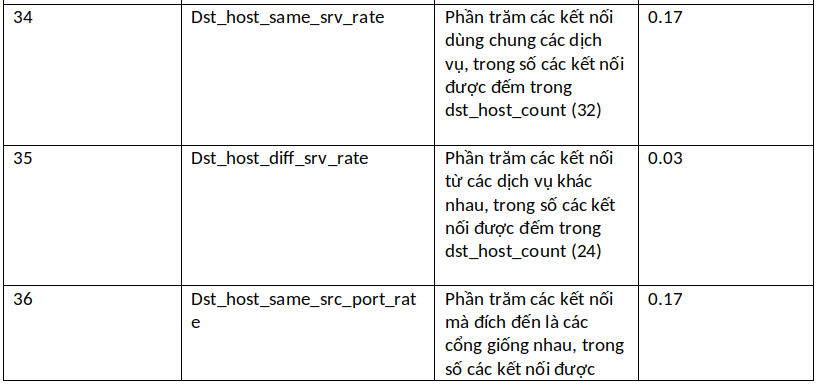
\includegraphics[scale=0.5]{table8}
	\label{fig:x cubed graph}
\end{figure}
\FloatBarrier
\begin{figure}[!htbp]
	\centering
	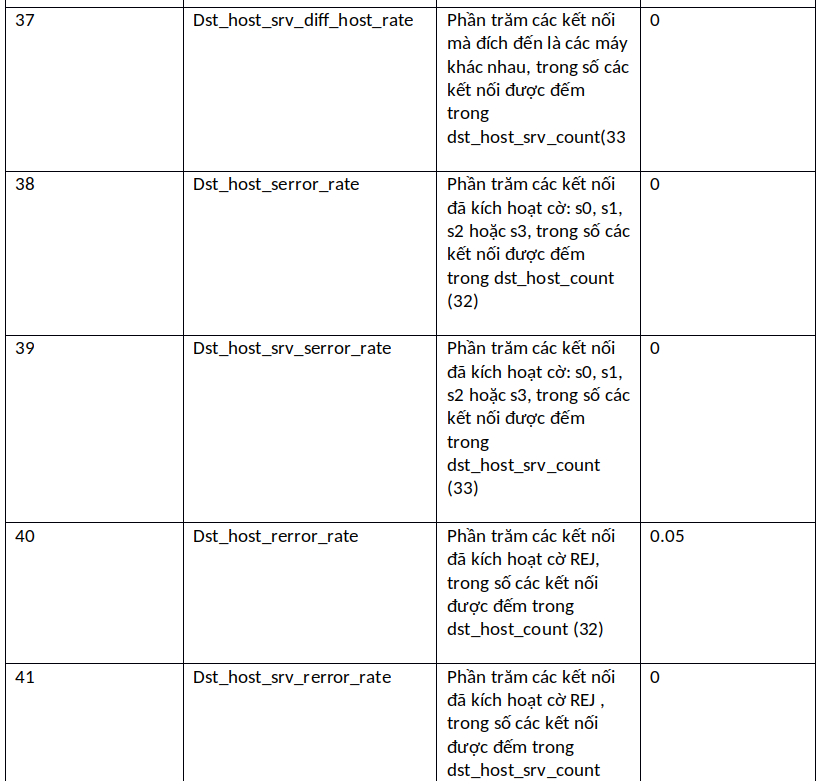
\includegraphics[scale=0.5]{table9}
	\label{fig:x cubed graph}
\end{figure}
\FloatBarrier

\begin{table}[!h]
	\begin{center}
		\begin{tabular}{ | c | c | }
			\hline
			\textbf{Loại}               & \textbf{Đặc tính} \\
			\hline
			\multirow{3}{2cm}{Nominal}  & protocol\_type(2) \\ &
			service(3)                                      \\ &
			flag(4)                                         \\
			\hline
			\multirow{10}{2cm}{Binary}  & land(7)           \\ &
			logged\_in(12)                                  \\ &
			root\_shell(14)                                 \\ &
			su\_attempted(15)                               \\ &
			is\_host\_login(21)                             \\ &
			is\_guest\_login(22)                            \\
			\hline
			\multirow{22}{2cm}{Numeric} & duration(1)       \\ &
			src\_bytes(5),                                  \\ &
			dst\_bytes(6)                                   \\ &
			wrong\_fragment(8)                              \\ &
			urgent(9)                                       \\ & hot(10) \\ &
			num\_failed\_logins(11)                         \\ &
			num\_compromised(13)                            \\ &
			num\_root(16)                                   \\ &
			num\_file\_creations(17)                        \\ &
			num\_shells(18)                                 \\ &
			num\_access\_files(19)                          \\ &
			num\_outbound\_cmds(20)                         \\ &
			count(23)
			srv\_count(24)                                  \\ &
			serror\_rate(25)                                \\ &
			srv\_serror\_rate(26)                           \\ &
			rerror\_rate(27)                                \\ &
			srv\_rerror\_rate(28)                           \\ &
			same\_srv\_rate(29)
			diff\_srv\_rate(30)                             \\ &
			srv\_diff\_host\_rate(31)                       \\ &
			dst\_host\_count(32)                            \\ &
			dst\_host\_srv\_count(33)                       \\ &
			dst\_host\_same\_srv\_rate(34)                  \\ &
			dst\_host\_diff\_srv\_rate(35)                  \\ &
			dst\_host\_same\_src\_port\_rate(36)            \\ &
			dst\_host\_srv\_diff\_host\_rate(37)            \\ &
			dst\_host\_serror\_rate(38)                     \\ &
			dst\_host\_srv\_serror\_rate(39)                \\ &
			dst\_host\_rerror\_rate(40)                     \\ &
			dst\_host\_srv\_rerror\_rate(41)                \\
			\hline
		\end{tabular}

	\end{center}
	\caption{Bảng phân loại các đặc tính \cite{machinelearning}}
	\label{table:1}
\end{table}
\FloatBarrier

\subsection{Phân nhóm}
Các lớp tấn công có trong bộ dữ liệu NSL-KDD được nhóm thành bốn loại:
\begin{enumerate}
	\item \textbf{DOS}: Từ chối dịch vụ là một thể loại tấn công, làm cạn kiệt tài nguyên của nạn nhân qua đó khiến cho nó không thể xử lý các yêu cầu hợp pháp - ví dụ: syn flood.
	      Các mục có liên quan: “byte nguồn” và “tỷ lệ phần trăm của gói có lỗi ”
	\item \textbf{Probing}: Mục tiêu của cuộc tấn công giám sát và thăm dò khác là thu thập thông tin về nạn nhân từ xa, ví dụ: quét cổng.
	      Các mục có liên quan: “thời lượng kết nối” và “byte nguồn”
	\item \textbf{U2R}: quyền truy cập trái phép vào đặc quyền người dùng (root) cục bộ là một kiểu tấn công, mà kẻ tấn công sử dụng tài khoản thông thường để đăng nhập vào hệ thống nạn nhân và cố gắng giành quyền root / quản trị viên bằng cách khai thác một số lỗ hổng trong nạn nhân.
	      Các cuộc tấn công tràn bộ đệm. Các tính năng liên quan: “số lượng tệp được tạo” và “số lời nhắc shell được gọi,”
	\item \textbf{R2L}: truy cập trái phép từ một máy từ xa, kẻ tấn công xâm nhập vào một máy từ xa và truy cập nội bộ của máy nạn nhân.
	      Ví dụ: đoán mật khẩu. Các tính năng liên quan: Tính năng ở cấp mạng - "thời lượng kết nối" và "dịch vụ được yêu cầu" và các tính năng ở cấp máy chủ - "số lần đăng nhập không thành công"
\end{enumerate}